%!TeX root = ../main.tex
% Add the above to each chapter to make compiling the PDF easier in some editors.

\chapter{Background}\label{chapter:Background}

\section{HPC}

High-performance computing, abbreviated as HPC, leverages the compute capacity of supercomputers or computer clusters to solve problems that are highly complex in nature.~\parencite{ibm_what_nodate} A computer cluster consists of many different computers (nodes) that are interconnected with high-speed, low-latency interconnects. Each node contains the same primary components a desktop or laptop PC would contain, such as a CPU, RAM, and storage. ~\parencite{iowa_state_university_what_nodate} It should be noted that modern CPUs, especially ones utilized in HPC applications, usually contain multiple physical cores and multiple threads to enable some amount of parallel processing. [example maybe?] Some nodes, just like some PCs, also have a dedicated GPU to accelerate certain types of workloads. ~\parencite{iowa_state_university_what_nodate}
 
\section{PCI-Express}
PCIe, or PCI-Express, shorthand for Peripheral Component Interconnect Express, is a "general-purpose serial I/O interconnect".~\parencite{pci-sig_pci_2011} PCIe, as an interface, allows the CPU to connect with, as the name suggests, peripherals and components.~\parencite{pcmag_definition_nodate} Common components and peripherals include, but are not limited to: Graphics cards, sound cards, video capture cards, WiFi cards, and storage.
PCIe is designed to replace the ageing PCI (Peripheral Component Interconnect), PCI-X (Peripheral Component Interconnect Extended), and AGP (Accelerated Graphics Port) standards.~\parencite{verma_pcie_2017} These standards are developed, defined, and maintained by the PCI-SIG group, which is a nonprofit organization with 800+ member companies based in Beaverton, Oregon.~\parencite{pci-sig_contact_nodate} This chapter will briefly introduce the key features and functionality of PCI-Express.

\subsection{Key Features}

PCI-Express is, at its core, a serialized, point-to-point connection that is designed to be processor agnostic, scalable, and backwards compatible with PCI.\cite{lawley_understanding_2014, pci-sig_pci_2011, pci-sig_membership_nodate} PCI-Express utilizes a dual-simplex connection to facilitate sending and receiving information concurrently. Additionally, to ensure backwards compatibility with PCI, PCI-Express shares the same memory configuration as PCI, which will be elaborated further upon in section \ref{sec:memory}. Further key features include better error handling and data integrity capabilities. \parencite{verma_pcie_2017} To future-proof the standard, current and future generations of PCIe are to be designed to be compatible with current PCIe standards.~\parencite{pci-sig_membership_nodate} So far, each generation of PCIe doubled the previous generation's theoretical maximum bandwidth, as seen in Table \ref{tab:bandwidths}.

\begin{table}
\includegraphics[width = \linewidth]{figures/PCIE-bandwidths}
\caption{PCI Express aggregate bandwidths by generation and link width ~\parencite{jackson_pci_2012}}
\label{tab:bandwidths}
\end{table}

\subsection{Functionality}

\subsubsection{packet}
PCIe, similar to IPv4 or IPv6, utilizes packets to communicate between the host - the CPU - and the device. As shown in figure \ref{fig:packet}, the packet consists of a few different elements, which will be further expanded upon below. 

\begin{figure}
\includegraphics[width = \linewidth]{figures/PCIE-packet}
\caption{An example of a PCI-Express packet ~\parencite{lawley_understanding_2014}}
\label{fig:packet}
\end{figure}

\begin{itemize}
\item Start: this is the start component which signals the begin of a packet to the physical layer.
\item Sequence: This two-byte sequence is used by the Data Link Layer to determine the sequence of the packets.
\item Header: The 12 to 16 Byte header will be discussed in further detail in subsection \ref{sec:header}. This component belongs to the Transaction layer. 
\item Payload: The PCIe payload. This is optional, however any memory transferred via memory copy operations will have the memory as payload. This also is a part of the Transaction layer.
\item ECRC: a CRC code for error-checking purposes used by the transaction layer.
\item LCRC: a CRC code for error-checking purposes used by the Data Link Layer.
\end{itemize}

[question: do i need a source for each of the bullet points? additionally, the source doesn't outright state that 'this is what this is for', in a degree, but it is inferred knowledge. what should I do about this?]

\subsubsection{header}
\label{sec:header}
As with IPv4 or IPv6, PCI-Express uses headers to determine the purpose and target of each TLP (Transaction Layer Packet)
However, instead of using IP-addresses, stored in the header, to determine the sender and the receiver, PCIe uses the Requester ID to determine the sender. The Address determines the receiver of the intended packet, as the device memory is memory-mapped into the host address domain to enable the processor's native load or store instructions to work with PCIe devices.~\parencite{oracle_inc_pci_nodate} As seen in Figure \ref{fig:header}, the header has a fixed format, similar to an IPv4 or v6 header. The fields and their uses are briefly explained below.

\begin{figure}
\includegraphics[width = \linewidth]{figures/PCIE-header}
\caption{An example of a memory request header ~\parencite{lawley_understanding_2014}}
\label{fig:header}
\end{figure}


\begin{itemize}
\item TC: Traffic Class: this denotes the priority of the packet. A larger value represents a higher priority.~\parencite{jackson_pci_2012}
\item TD: The TLP Digest field. If TD is set to 1, it indicates that there is additional CRC data in the TLP data. [cite xillybus]
\item Length: more or less self-explanatory: length denotes the length of the payload in Double Words. [cite xillybus]
\item Requester ID: self-explanatory: the ID of the device that requested or sent the packet. [cite xillybus]
\item Tag: The Tag field has the function of a tracking number, as for read requests, the device must copy this value to its response. All outstanding tags must be unique to ensure data integrity. [cite xillybus]
\item DW BE fields: DW BE stands for Double-Word Byte Enable. This denotes which of the bytes in the first / last DWs are valid. [cite xillybus]
\item Address: self-explanatory: The Address to which this packet is addressed, as explained above. Additionally, for read and write requests, this denotes the starting address of the read or write. [cite xillybus]
\item The EP and Attr fields are not further elaborated upon as they are rarely used by PCIe endpoint devices. [cite xillybus]
\end{itemize}

[todo: update and verify with book]

\subsection{Topology and Communication}

\subsubsection{Topology}
There are four significant components to be mentioned when discussing the topology of a PCI-Express based system. PCIe endpoints, switches, bridges, and a root complex. 
The communication between CPU cores and memory controllers to the PCIe endpoint is handled by the PCIe root complex. This communication can be routed through (but does not require) PCIe switches. PCIe switches allow for cascading connections, however do not benefit the total bandwidth, which is limited by the PCIe root complex in a CPU.~\parencite{nakamura_thorough_2017}
Bridges are used to connect legacy PCI and PCI-X devices with the PCIe root complex.~\parencite{pci-sig_pci_2011}
Figure \ref{fig:topology} shows an example PCIe configuration of an Intel-based processor.

\begin{figure}
\includegraphics[width = \linewidth]{figures/PCIE-topology}
\caption{PCIe configuration on an Intel-based system\cite{nakamura_thorough_2017}}
\label{fig:topology}
\end{figure}
\subsubsection{Memory Management}
\label{sec:memory}

The PCIe memory structure is, due to compatibility reasons, the same as the memory structure found in the older PCI standard. This divides the device memory into three major parts for addressing:\cite{jackson_pci_2012}
\begin{itemize}
\item Configuration
\item Memory
\item IO
\end{itemize}

The configuration address space enables software to both identify and correctly configure the device, and is defined by its physical bus and device number.\cite{oracle_inc_pci_nodate}

The memory address space is where the storage and registers of a PCIe device is mapped.\cite{jackson_pci_2012} This memory space is also memory-mapped to the host address domain for ease of access by the CPU.\cite{oracle_inc_pci_nodate}

The IO address space is a place dedicated to accessing the internal registers / storage of a PCIe or PCI device. However, this is mostly deprecated in PCIe as the internal registers and storage of said devices are simply mapped into the memory address space instead. It is now common practice to map the same set of registers in both memory and IO address space for backwards compatibility purposes. The PCIe specification discourages use of the IO space, which indicates that it remains solely for legacy support purposes.\cite{jackson_pci_2012}

\subsubsection{Links and Lanes}
A connection between the two PCIe devices is called a link, which is made up of lanes. \cite{jackson_pci_2012} A PCIe device, in this case, can be the CPU's PCIe root complex, bridges, switches, or a PCIe end point. A lane, on the hardware level, is a set of four copper wires, two for each signal direction.\cite{jackson_pci_2012} Due to the scalability of PCIe, the amount of lanes in a link is variable, from 1 up to 32, and is represented by a x in front of the lane width, e.g. PCIe x16, which indicates that the PCIe link has 16 lanes. A wider link means higher bandwidths and transmit capabilities, however it also means higher power consumption, space, and cost. \cite{jackson_pci_2012} Figure \ref{fig:link} illustrates an example PCIe link with several lanes.


\begin{figure}
\begin{center}
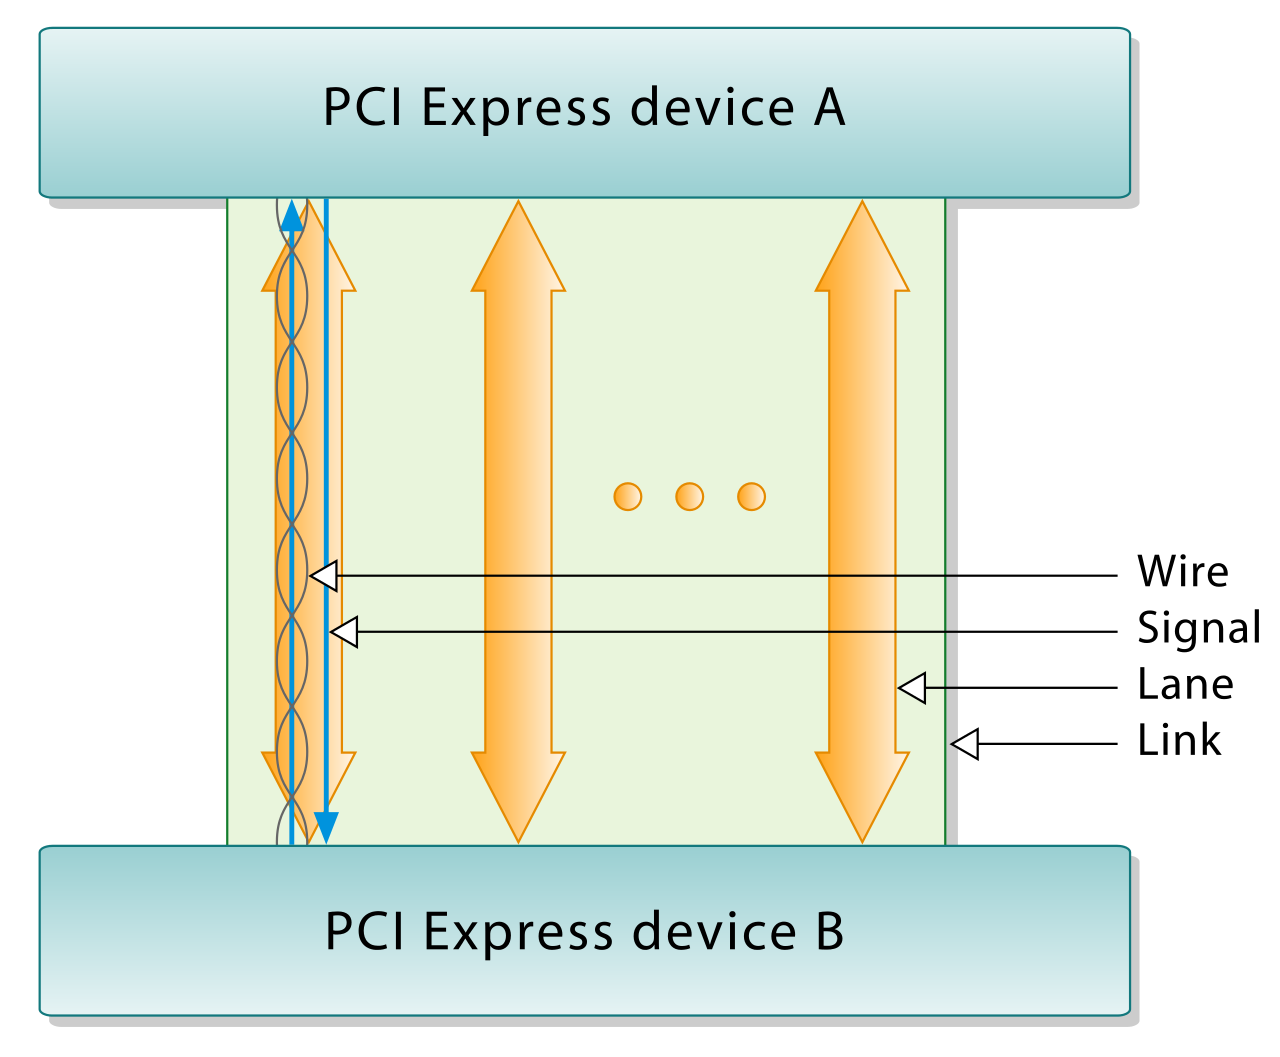
\includegraphics[height = 200px]{figures/PCIE-link}
\caption{An example PCIe link between two devices \cite{budruk_pci_2014}}
\label{fig:link}
\end{center}
\end{figure}

\subsection{Revisions and Further Specifications}

PCI-Express was first introduced in 2003, and has received a new revision once every three to four years on average. Whilst most current hardware uses PCIe 3.0 and 4.0, introduced in 2010 and 2017 respectively [does this need a source?], PCI-SIG has already published their specifications for the PCIe 5.0 and 6.0 standards. These, again, double the bandwidths of the previous generation, enabling theoretical transfer speeds of up to 128GB/sec in both directions on a PCIe 6.0 x16 link.\cite{sharma_pci_2020} However, it is to be expected that these high-speed interconnect standards will take a few years to become widely available and adopted, as Intel only released their first PCIe 5.0-capable CPUs around the end of 2021. \cite{intel_product_nodate} Additionally, other manufacturers and companies have developed their own protocols and standards to extend the feature-set of PCIe, such as Intel's Thunderbolt, which enables PCIe devices to be connected externally with only a small loss of performance. \cite{intel_what_nodate} Another example is the NVMe standard, a PCIe-compatible interface specifically devised and optimized for high-bandwidth, low-latency storage solutions. \cite{kingston_understanding_nodate}


\section{Graphics Processing Units}


\subsection{What are GPUs}
To begin with, it should be noted that the term graphics processing unit (GPU) does not equate to a graphics card. A GPU is a specialized processing unit primarily designed for parallel processing and accelerating workloads that require parallel processing. \cite{intel_what_nodate} A graphics card, on the other hand, is the add-in card that features a PCI-Express link to facilitate communication between CPU and GPU, dedicated memory and power delivery for the GPU, and the GPU itself. It should also be noted that the graphics card usually has its own dedicated PCB. [does this need citing?] There are also integrated GPUs, which can be embedded alongside the CPU.  These integrated GPUs are usually less powerful compared to discrete GPUs. \cite{intel_what_nodate}

\subsection{Uses of GPUs}

GPUs originally began as, as their names suggest, dedicated graphics accelerators optimized for floating-point operations, which are essential to 3D graphics rendering. They were initially developed as a hardware pipeline with fixed functionality, namely to render graphics. Over the years, GPU architecture has evolved from essentially being an integrated frame buffer into a set of general-purpose, highly parallel, programmable processing cores, enabling more general-purpose computation. ~\parencite{mcclanahan_history_2010} Today, a GPU is more of an accelerator for many different use-cases and workloads. Examples include, for personal use, gaming, video editing, and content creation. \cite{intel_what_nodate} On the scientific side, GPUs are frequently used to accelerate workloads that require parallel computing, such as machine learning, fluid dynamics, and data science. \cite{nvidia_cuda_2017}


\subsection{GPU Memory}
Addressing GPU memory, assuming that the GPU is connected via PCI-Express and has its own dedicated video memory, works in the same way as addressing memory in other PCIe devices, which was briefly touched upon in section \ref{sec:memory}. However, GPU memory usually has higher throughput bandwidths compared to conventional RAM of a similar period. As example, current top of the line graphics cards from Nvidia are equipped with GDDR6X memory, which has a theoretical maximum system bandwith of one terabyte per second.~\cite{nvidia_nvidia_nodate, micron_technology_inc_ram_nodate} On the other hand, state of the art main memory, currently DDR4, is limited to a bandwidth of about 35 gigabytes per second.~\cite{micron_technology_inc_ram_nodate}

TODO: DDR5 standard, however: numbers hard to find. what to put?


\section{CUDA}

CUDA is a closed source API developed and maintained by Nvidia for general-purpose GPU computing for their GPUs and graphics cards. It is designed to work with C++ and Fortran and comes with a set of GPU-accelerated libraries, optimization tools, debugging tools, and a C++ compiler.~\parencite{nvidia_cuda_2017} Some sample libraries include: linear algebra, signal processing, and image processing. \parencite{nvidia_cuda_2020} For this thesis, only the C++ version of CUDA is discussed in further detail.


\subsection{Kernels and Scalability}
CUDA uses kernels, which are an extension to standard C++ functions. Kernels, when called, are executed N times by N different threads, and enable these threads to run on the GPU. This enables heterogeneous programming, which allows serial code to run on the host - the CPU - and parallel code, the kernels, to run on the GPU, thereby leveraging the GPU's increased capabilities for parallel computing to accelerate the workload. The kernel is executed on a thread, many of which make up a block, many of which, in return, make up a grid, the dimensions of which are defined upon calling the kernel. Different blocks can be executed in parallel, or in sequence, in any order, on any of the multiprocessors of a GPU, which enables automatic scalability as the compiled program can run irrespective of the amount of multiprocessors present on the GPU.~\parencite{nvidia_cuda_nodate}


\subsection{Memory Management}
CUDA assumes that the CPU and GPU maintain separate memory spaces, and is able to manage both host and device memory. CUDA can both manage shared memory, which is visible and accessible for both the CPU and GPU, and dedicated device memory, which is not accessible by the CPU. CPU memory is, unless overridden by CUDA, managed natively by C++. Memory management includes allocation, deallocation, and data transfer.~\parencite{nvidia_cuda_nodate}

[maybe extend this section a bit? Not sure if i covered everything]
[add sources]
[maybe add graphics]



